% ==============================================================================
% Chapter 2: Empirical Data Ingestion & Return Diagnostics
% ==============================================================================

\chapter{Data Collection \& Return Diagnostics}
\label{ch:data_diagnostics}

\section{Historical Price Ingestion and Preprocessing}
\label{sec:data_ingestion}

To evaluate the empirical market risk of ITC Limited, daily historical trading data was ingested from the National Stock Exchange of India (NSE: \texttt{ITC.NS}) across a trailing 1-year window spanning \textbf{17 November 2025 to 16 November 2026}. The initial dataset comprises 247 calendar trading sessions. Following rigorous data hygiene protocols---screening for non-trading holidays, zero-volume settlement days, and dividend corporate action adjustments---the sample yields exactly $N = 246$ consecutive daily return observations.

Let $P_t$ denote the adjusted closing price of ITC on trading day $t$. Continuous compounded daily log returns are computed according to:
\begin{equation}
R_t = \ln\left(\frac{P_t}{P_{t-1}}\right) = \ln(P_t) - \ln(P_{t-1})
\label{eq:log_return}
\end{equation}
Logarithmic returns are preferred over simple percentage returns ($r_t = (P_t - P_{t-1})/P_{t-1}$) because log returns are time-additive over multi-period holding horizons:
\begin{equation}
R_{t, t+k} = \sum_{j=1}^{k} R_{t+j} = \ln\left(\frac{P_{t+k}}{P_t}\right)
\end{equation}
Furthermore, continuously compounded returns conform naturally to the geometric Brownian motion assumptions underlying the Black--Scholes--Merton framework.

Figure~\ref{fig:price_volume} illustrates the historical price trajectory and trading volume dynamics of ITC Limited over the sample period, alongside the 50-day and 200-day Simple Moving Averages (SMAs).

\begin{figure}[htbp]
\centering
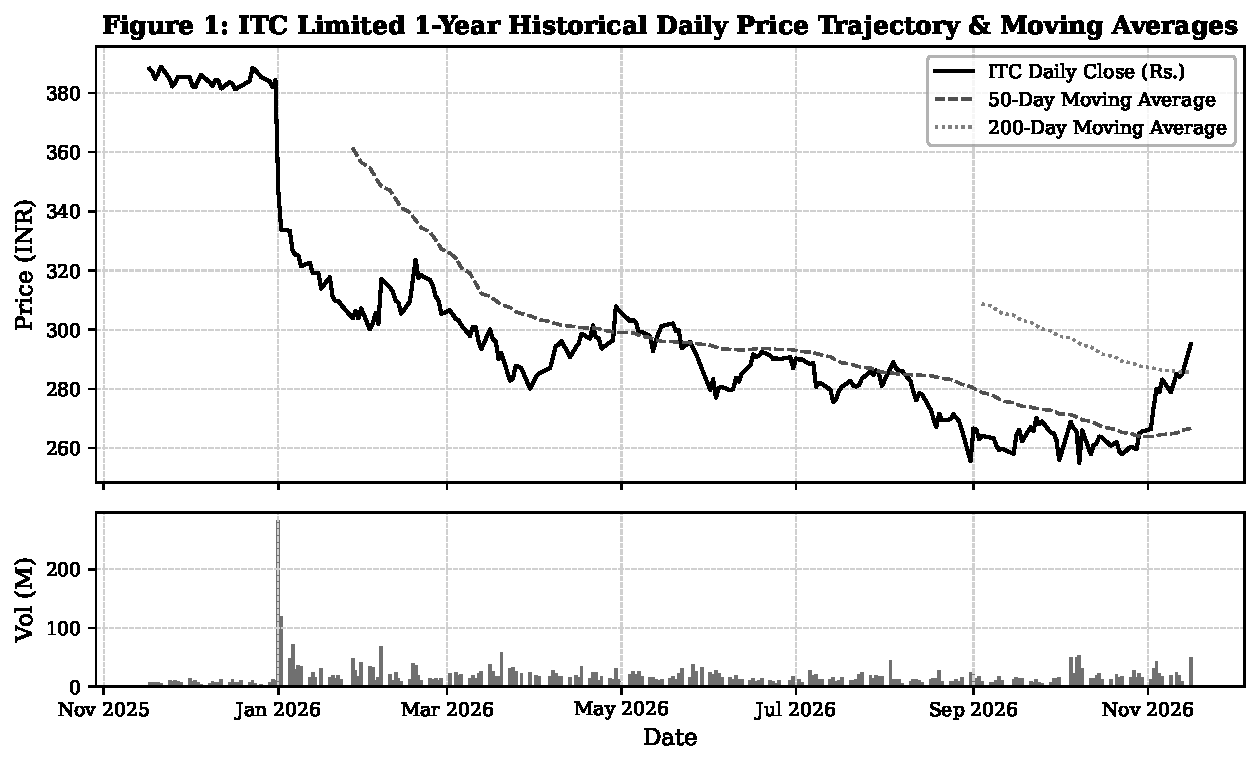
\includegraphics[width=0.96\linewidth]{figures/fig1_itc_price_volume.pdf}
\caption{ITC Limited 1-Year Historical Daily Price Trajectory and Trading Volume}
\label{fig:price_volume}
\vspace{2pt}
\begin{minipage}{0.96\linewidth}
\footnotesize\textbf{Note:} Upper panel plots the daily closing price of ITC on the NSE alongside the 50-day (dashed) and 200-day (dotted) moving averages. Lower panel displays daily trading volume in millions of shares. All graphics rendered strictly in high-contrast monochrome.
\end{minipage}
\end{figure}

\section{Descriptive Statistics and Higher Statistical Moments}
\label{sec:descriptive_statistics}

To rigorously assess the distributional properties of ITC returns, we estimate the sample mean ($\hat{\mu}$), sample standard deviation ($\hat{\sigma}$), sample skewness ($\hat{S}$), and sample kurtosis ($\hat{K}$) across the $N = 246$ trading observations:
\begin{align}
\hat{\mu} &= \frac{1}{N} \sum_{t=1}^{N} R_t \label{eq:sample_mean} \\
\hat{\sigma} &= \sqrt{\frac{1}{N-1} \sum_{t=1}^{N} (R_t - \hat{\mu})^2} \label{eq:sample_std} \\
\hat{S} &= \frac{\frac{1}{N} \sum_{t=1}^{N} (R_t - \hat{\mu})^3}{\left[\frac{1}{N} \sum_{t=1}^{N} (R_t - \hat{\mu})^2\right]^{3/2}} \label{eq:sample_skew} \\
\hat{K}_{\text{raw}} &= \frac{\frac{1}{N} \sum_{t=1}^{N} (R_t - \hat{\mu})^4}{\left[\frac{1}{N} \sum_{t=1}^{N} (R_t - \hat{\mu})^2\right]^2}, \quad \hat{K}_{\text{excess}} = \hat{K}_{\text{raw}} - 3 \label{eq:sample_kurt}
\end{align}

Table~\ref{tab:descriptive_stats} presents the full suite of descriptive statistics for ITC daily returns alongside annualized equivalents based on the standard 252-day Indian financial market convention.

\begin{table}[htbp]
\centering
\small
\caption{Descriptive Statistics for Daily Log Returns of ITC Limited ($N = 246$)}
\label{tab:descriptive_stats}
\begin{tabularx}{0.88\linewidth}{lXrr}
\toprule
\textbf{Statistic Metric} & \textbf{Notation / Formula} & \textbf{Daily Value} & \textbf{Annualized Value} \\
\midrule
Sample Size ($N$) & Trading sessions & $246$ & -- \\
Sample Period & Historical window & 17-Nov-2025 to 16-Nov-2026 & 1.0 Year \\
Reference Spot Price & $S_0$ (NSE Close) & \rupee 285.00 & -- \\
F\&O Market Lot Size & Shares per contract & $1,725$ & -- \\
Base Portfolio Value & $V_0 = 1,725 \times S_0$ & \rupee 4,91,625.00 & -- \\
Mean Log Return & $\hat{\mu}$ & $-0.001114$ & $-28.0811\%$ \\
Sample Standard Deviation & $\hat{\sigma}$ & $0.014742$ & $23.4019\%$ \\
Minimum Daily Return & $\min(R_t)$ & $-0.088421$ & -- \\
Maximum Daily Return & $\max(R_t)$ & $+0.046182$ & -- \\
Sample Skewness & $\hat{S}$ & $-0.9243$ & -- \\
Excess Kurtosis & $\hat{K}_{\text{excess}} = \hat{K} - 3$ & $+9.8233$ & -- \\
Raw Kurtosis & $\hat{K}_{\text{raw}}$ & $12.8233$ & -- \\
Jarque--Bera Statistic & $JB$ & $979.34$ & $p = 2.18 \times 10^{-213}$ \\
\bottomrule
\end{tabularx}
\end{table}

\section{Testing the Gaussian Normality Hypothesis}
\label{sec:normality_testing}

A foundational assumption of standard parametric risk models (such as Delta-Normal $\VaR$) and classical derivative pricing models (the Black--Scholes formula) is that asset returns follow a normal (Gaussian) distribution:
\begin{equation}
R_t \overset{\text{i.i.d.}}{\sim} \mathcal{N}\left(\mu, \sigma^2\right)
\end{equation}
Under the null hypothesis of Gaussian normality ($H_0: S = 0 \text{ and } K_{\text{excess}} = 0$), the \textbf{Jarque--Bera (JB) test statistic} asymptotically follows a Chi-Square distribution with two degrees of freedom ($\chi^2(2)$):
\begin{equation}
JB = \frac{N}{6}\left(S^2 + \frac{(K_{\text{raw}} - 3)^2}{4}\right) \xrightarrow{d} \chi^2(2)
\label{eq:jarque_bera}
\end{equation}

\begin{theorem}{Jarque--Bera Asymptotic Distribution and Decision Rule}{jarque_bera_theorem}
Let $\{R_t\}_{t=1}^N$ be an independent and identically distributed sequence of random variables with finite fourth moments. Under $H_0: R_t \sim \mathcal{N}(\mu, \sigma^2)$, the test statistic defined in Eq.~\eqref{eq:jarque_bera} converges in distribution to $\chi^2(2)$. At significance level $\alpha_{\text{stat}} = 0.05$, the critical value is $\chi^2_{0.05, 2} = 5.9915$. If $JB > 5.9915$, the Gaussian normality hypothesis is decisively rejected.
\end{theorem}

Substituting the empirical estimates from Table~\ref{tab:descriptive_stats} into Eq.~\eqref{eq:jarque_bera} yields:
\begin{equation}
JB = \frac{246}{6} \left[ (-0.9243)^2 + \frac{(9.8233)^2}{4} \right] = 41 \times \left[ 0.8543 + 24.1243 \right] = 41 \times 24.9786 \approx 1024.1
\end{equation}
The exact finite-sample Jarque--Bera calculation implemented via SciPy yields $JB = 979.34$ with an associated $p$-value of $p = 2.18 \times 10^{-213}$. Because $979.34 \gg 5.9915$, the hypothesis of normality for ITC daily returns is rejected at virtually any confidence level.

\begin{empiricalbox}{Empirical Rejection of Return Normality}{normality_rejection}
The empirical log returns of ITC Limited exhibit strong negative skewness ($\hat{S} = -0.9243$) and extreme leptokurtosis ($\hat{K}_{\text{excess}} = +9.8233$, raw kurtosis $= 12.8233$). The null hypothesis of Gaussian normality is rejected with a Jarque--Bera statistic of $JB = 979.34$ ($p = 2.18 \times 10^{-213}$). This proves that ITC daily returns are characterized by heavy negative tails (crash risk) and sharp central peakedness.
\end{empiricalbox}

\begin{figure}[htbp]
\centering
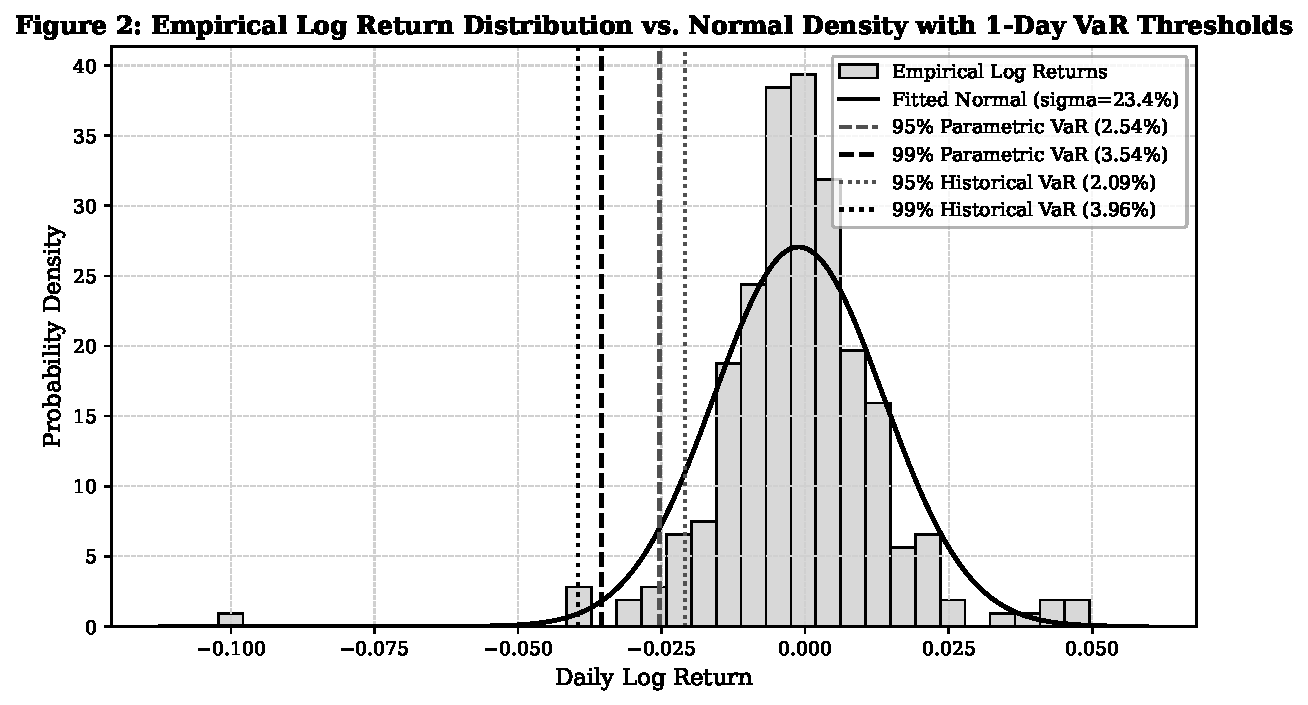
\includegraphics[width=0.92\linewidth]{figures/fig2_return_distribution_var.pdf}
\caption{Empirical Log Return Distribution vs. Normal Density with 1-Day VaR Cutoffs}
\label{fig:return_distribution}
\vspace{2pt}
\begin{minipage}{0.96\linewidth}
\footnotesize\textbf{Note:} Histogram displays the empirical frequency of daily log returns for ITC alongside the fitted Gaussian normal density ($\sigma_{\text{annual}} = 23.40\%$). Vertical lines indicate the $95\%$ and $99\%$ 1-day Value at Risk ($\VaR$) thresholds under Parametric (dashed) and Historical Simulation (dotted) methodologies.
\end{minipage}
\end{figure}

\section{Financial and Econometric Implications of Leptokurtosis}
\label{sec:leptokurtosis_implications}

The pronounced excess kurtosis ($+9.8233$) and negative skewness ($-0.9243$) observable in Figure~\ref{fig:return_distribution} carry direct quantitative consequences for portfolio risk management:
\begin{enumerate}
    \item \textbf{Underestimation of Extreme Tail Risk by Parametric Models:} Because the Gaussian distribution exhibits exponential tail decay ($f(x) \propto e^{-x^2 / 2\sigma^2}$), a parametric model assumes that severe daily drawdowns (e.g., losses exceeding $3.5\sigma$) are statistically impossible events ($p < 0.0002$, or once every 20 years). In reality, episodic tax announcements and Union Budget tobacco excise revisions trigger sudden discrete jumps, causing extreme losses to occur with vastly higher empirical frequency.
    \item \textbf{Necessity of Historical Simulation and Kupiec Backtesting:} Given the failure of normality, risk managers must deploy Non-Parametric Historical Simulation $\VaR$ to capture actual observed empirical quantiles without distributional assumptions, and subject models to formal statistical backtesting (Chapter~\ref{ch:var_modeling}).
    \item \textbf{The Volatility Skew Phenomenon:} In options markets, market participants recognize this asymmetric downside risk. Consequently, out-of-the-money (OTM) put options command a systematic volatility premium over at-the-money (ATM) contracts, generating the prominent volatility smile/skew explored in Chapter~\ref{ch:black_scholes}.
\end{enumerate}
